% !TEX program = pdflatex
\documentclass[dvipsnames,aspectratio=169,handout]{beamer}
\usepackage{tikz,amsfonts}
% xcolor is typically loaded by beamer; re-loading with options may cause an option clash.
\usepackage{xcolor}
\usetikzlibrary{arrows,arrows.meta,positioning,calc,shapes}
\usepackage[absolute,overlay]{textpos}
\usepackage{multirow}
\usepackage{environ,lipsum}
\usepackage{listings}



\lstset{ 
  language=R,                     % the language of the code
  basicstyle=\scriptsize\ttfamily, % the size of the fonts that are used for the code
  columns=fullflexible,
%  numbers=left,                   % where to put the line-numbers
%  numberstyle=\tiny\color{Blue},  % the style that is used for the line-numbers
%  stepnumber=1,                   % the step between two line-numbers. If it is 1, each line
                                  % will be numbered
%  numbersep=5pt,                  % how far the line-numbers are from the code
  backgroundcolor=\color{Dandelion!15!white},  % choose the background color. You must add \usepackage{color}
  showspaces=false,               % show spaces adding particular underscores
  showstringspaces=false,         % underline spaces within strings
  showtabs=false,                 % show tabs within strings adding particular underscores
  frame=single,                   % adds a frame around the code
  rulecolor=\color{Dandelion!15!white},        % if not set, the frame-color may be changed on line-breaks within not-black text (e.g. commens (green here))
  tabsize=2,                      % sets default tabsize to 2 spaces
  captionpos=b,                   % sets the caption-position to bottom
  breaklines=true,                % sets automatic line breaking
  breakatwhitespace=false,        % sets if automatic breaks should only happen at whitespace
  keywordstyle=\color{RoyalBlue!80!black},      % keyword style
  commentstyle=\color{YellowGreen!60!black},   % comment style
  %stringstyle=\color{ForestGreen}      % string literal style
} 
\lstset{alsoletter={.,_}, morekeywords={cor.test,set.seed,dcor.test,make_tree,sample_gnm,graph,ci.test,qgraph,sample_smallworld,ciTest_table,IsingFit,averageLayout,read.table,install.packages,bdgraph,stepwise,dmod,cmod,ciTest,graph_from_adjacency_matrix,mvrnorm,CondIndTest,as.data.frame,chisq.test,gnm,smallworld,ug,dag,edge,as.igraph,degree,diameter,centrality,cluster,betweenness,at}
}


\newcommand{\customframefont}[1]{
\setbeamertemplate{itemize/enumerate body begin}{#1}
\setbeamertemplate{itemize/enumerate subbody begin}{#1}
}

\NewEnviron{framefont}[1]{
\customframefont{#1} % for itemize/enumerate
{#1 % For the text outside itemize/enumerate
\BODY
}
\customframefont{\normalsize}
}



%%%%%%%%% BASICS
\usenavigationsymbolstemplate{}

\setbeamertemplate{frametitle}
  {\begin{centering}\smallskip
   \insertframetitle\par
   \smallskip\end{centering}}
\setbeamersize{text margin left=.2cm,text margin right=.2cm} 
\setbeamertemplate{itemize item}{$\bullet$}
\setbeamertemplate{navigation symbols}{}
\setbeamertemplate{footline}[text line]{%
    \hfill\strut{%
        \scriptsize\sf\color{black!60}%
        \quad\insertframenumber/\inserttotalframenumber
    }%
    \hfill
    
}

%%%%%%%%% COLOR THEME

% Define some colors:
\definecolor{asparagus}{rgb}{0.53, 0.66, 0.42}
\definecolor{DarkFern}{HTML}{407428}
\definecolor{DarkCharcoal}{HTML}{4D4944}
\colorlet{Fern}{DarkFern!85!white}
\colorlet{Charcoal}{DarkCharcoal!85!white}
\colorlet{LightCharcoal}{Charcoal!50!white}
\definecolor{Important}{RGB}{234,122,133}
\colorlet{AlertColor}{Melon!30!red}
\colorlet{DarkRed}{red!70!black}
\colorlet{DarkBlue}{blue!70!black}
\colorlet{DarkGreen}{green!70!black}
\definecolor{ExampleBlue}{RGB}{230,242,255}
\setbeamercolor{examplepanel}{fg=black,bg=ExampleBlue}
% Use the colors:
\setbeamercolor{title}{fg=Fern}
\setbeamercolor{frametitle}{fg=Fern}
\setbeamercolor{normal text}{fg=Charcoal}
\setbeamercolor{block title}{fg=black,bg=Fern!15!white}
\setbeamercolor{block body}{fg=black,bg=Fern!15!white}
%\setbeamercolor{block body alerted}{fg=black,bg=Goldenrod!5!white}
%\setbeamercolor{block body example}{fg=black,bg=Fern!15!white}
\setbeamercolor{alerted text}{fg=AlertColor}
\setbeamercolor{itemize item}{fg=Charcoal}
\setbeamercolor{framesource}{fg=gray}
\setbeamerfont{framesource}{size=\tiny}

%%%%% DEFINITIONS

\DeclareMathOperator{\sgn}{sgn}
\DeclareMathOperator{\rank}{rank}
\DeclareMathOperator{\D}{D}
\DeclareMathOperator{\cov}{cov}
\DeclareMathOperator{\cor}{cor}
\DeclareMathOperator{\var}{var}
\DeclareMathOperator{\tr}{tr}
\DeclareMathOperator{\pa}{pa}
\DeclareMathOperator{\de}{de}
\DeclareMathOperator{\nd}{nd}

\newcommand{\bx}{\mathbf{x}}
\newcommand{\by}{\mathbf{y}}
\newcommand{\C}{\mathbb{C}}
\newcommand{\cC}{\mathcal{C}}
\newcommand{\E}{\mathbb{E}}
\newcommand{\cE}{\mathcal{E}}
\newcommand{\cI}{\mathcal{I}}
\newcommand{\J}{\rm {J}}
\newcommand{\cL}{\mathcal{L}}
\newcommand{\cM}{\mathcal{M}}
\newcommand{\N}{\mathbb{N}}
\renewcommand{\P}{\mathbb{P}}
\newcommand{\Q}{\mathbb{Q}}
\newcommand{\R}{\mathbb{R}}
\renewcommand{\S}{\mathbb{S}}
\newcommand{\cS}{\mathcal{S}}
\newcommand{\cX}{\mathcal{X}}
\newcommand{\Z}{\mathbb{Z}}
\newcommand{\bs}{\boldsymbol}
\newcommand{\imp}[1]{\textcolor{DarkRed}{\textbf{#1}}}
\newcommand{\why}{\textcolor{WildStrawberry}{{\textsc{why?}}}}
\newcommand{\indep}{\mbox{\,$\perp\!\!\!\perp$\,}}
\newcommand{\mtp}{{\rm MTP}_{2}}
\newcommand{\eps}{\varepsilon}

\def\imagetop#1{\vtop{\null\hbox{#1}}}
\def\house{\hbox{\kern3pt \vbox to12pt{}% 
   \pdfliteral{q 0 0 m 0 5 l 5 10 l 10 5 l 10 0 l 7 0 l 7 5 l 3 5 l 3 0 l f
               1 j 1 J -2 5 m 5 12 l 12 5 l S Q }%
   \kern 13pt}}

%source for images
\newcommand{\source}[1]{\begin{textblock*}{4cm}(8.7cm,8.6cm)
    \begin{beamercolorbox}[ht=0.5cm,right]{framesource}
        \usebeamerfont{framesource}\usebeamercolor[fg]{framesource} Source: {#1}
    \end{beamercolorbox}
\end{textblock*}}

%%% TITLE INFO



\institute{\begin{center}
  \IfFileExists{LOGOstats.png}{\raisebox{-0.5\height}{
\includegraphics[scale=.27]{LOGOstats.png}}}{} 
  \hspace{1mm}
  \IfFileExists{LOGOBSE.jpg}{\raisebox{-0.5\height}{
\includegraphics[scale=.08]{LOGOBSE.jpg}}}{} 
\end{center}}


\setbeamercolor{notabene}{fg=black!50!white,bg=Gray!10!white}
\setbeamercolor{important}{fg=red!50!white,bg=red!7!white}
\setbeamercolor{goldbox}{fg=black!50!white,bg=Goldenrod!7!white}
\setbeamercolor{result}{fg=black!60!white,bg=OliveGreen!4!white}
% \begin{beamercolorbox}[wd=\paperwidth,sep=7pt]{important}	
%	%\end{beamercolorbox}


\title{Advanced techniques in applied economics}
\subtitle{Lecture 5: Latent variable models --- from trees to neural nets}
\author{Piotr Zwiernik}
\date{Spring 2026}

\newcommand{\Cov}{\operatorname{Cov}}
\newcommand{\diag}{\operatorname{diag}}
\newcommand{\logit}{\operatorname{logit}}
\newcommand{\sech}{\operatorname{sech}}

\begin{document}

% ------------------------------------------------------------
% Title
% ------------------------------------------------------------

\begin{frame}
\titlepage
\end{frame}

% ------------------------------------------------------------
% Overview
% ------------------------------------------------------------

\section{Overview}

\begin{frame}[plain,noframenumbering]{}
\begin{center}
{\huge \textcolor{DarkRed}{Latent structure as hidden economic mechanism}}
\end{center}
\end{frame}

\begin{frame}{What changes today?}
In the previous lectures, graphs described dependence among \emph{observed} variables.
Today we allow some important variables to be \imp{hidden}.

\begin{columns}[T]
\begin{column}{0.53\textwidth}
\begin{block}{Why hidden variables?}
\begin{itemize}
    \item market-wide shocks are not directly observed,
    \item consumers or firms belong to hidden segments,
    \item hierarchical structures may be only partially measured.
\end{itemize}
\end{block}
\end{column}
\begin{column}{0.43\textwidth}
\begin{alertblock}{Dimension reduction}
	PCA and related models assume low-dim latent structure in the data.
\end{alertblock}
\begin{block}{Main question}
\vspace{-1mm}
Can a small number of latent variables explain complicated patterns in the data?
\end{block}
\end{column}
\end{columns}

\begin{beamercolorbox}[wd=\textwidth,sep=8pt,center,rounded=true,shadow=true]{important}
\textbf{Main message:}
latent variables can turn a complicated observed dependence pattern into a simple hidden structure.
\end{beamercolorbox}
\end{frame}

\begin{frame}{Roadmap for today}
\begin{enumerate}
    \item Factor analysis and hidden common factors
    \item Gaussian mixtures and latent classes
    \item Latent tree models and hierarchical structure
    \item Message passing / belief propagation intuition
    \item Restricted Boltzmann machines as a bridge to neural nets
\end{enumerate}

\vspace{2mm}
\begin{beamercolorbox}[wd=\textwidth,sep=7pt,center,rounded=true,shadow=true]{important}
When dependence is too complicated at the surface, look for a simpler hidden layer underneath.
\end{beamercolorbox}
\end{frame}

% ------------------------------------------------------------
% Factor analysis
% ------------------------------------------------------------

\section{Factor analysis}

\begin{frame}[plain,noframenumbering]{}
\begin{center}
{\Huge \textcolor{DarkRed}{Part 1: Factor analysis}}
\end{center}
\end{frame}

\begin{frame}{Why economists care about factor models}
\begin{columns}[T]
\begin{column}{0.48\textwidth}
\begin{block}{Finance}
A large collection of returns often moves because of a few common factors:
\begin{itemize}
    \item market return,
    \item sectoral shocks,
    \item liquidity or volatility factors.
\end{itemize}
\end{block}
\end{column}
\begin{column}{0.48\textwidth}
\begin{block}{Applied micro and macro}
\vspace{-2mm}
Latent variables can represent
\begin{itemize}
    \item ability,
    \item sentiment,
    \item business-cycle conditions,
    \item hidden household or firm types.
\end{itemize}
\end{block}
\end{column}
\end{columns}
\medskip

\begin{beamercolorbox}[wd=\textwidth,sep=7pt,center,rounded=true,shadow=true]{important}
A factor model says: many variables may comove because they are driven by the same hidden source.
\end{beamercolorbox}
\end{frame}

\begin{frame}{The factor analysis model}
The basic Gaussian factor model is
\[
X = \mu + WZ + \varepsilon,
\qquad
Z\sim N_r(0,I_r),
\qquad
\varepsilon\sim N_m(0,\Psi),
\qquad
Z\indep \varepsilon,
\]
where $\Psi$ is diagonal.

\begin{block}{Interpretation}
\begin{itemize}
    \item $Z\in\R^r$ are the latent factors,
    \item $W\in\R^{m\times r}$ is the loading matrix,
    \item $\Psi$ captures variable-specific noise not explained by the common factors.
\end{itemize}
\end{block}

\begin{alertblock}{Covariance form}
The induced covariance matrix is
\[
\Sigma = WW^\top + \Psi.
\]
So dependence is split into a low-rank common part and a diagonal idiosyncratic part.
\end{alertblock}
\end{frame}

\begin{frame}{A one-factor economic example}
Suppose $m$ observed returns satisfy
\[
X_i = \lambda_i F + \varepsilon_i,
\qquad i=1,\ldots,m,
\]
where $F$ is a latent factor, and all $\varepsilon_i$ independent and independent of $F$.
\begin{columns}[T]
\begin{column}{0.56\textwidth}
\begin{block}{Covariance implication}
For $i\neq j$,\\[1mm]
\qquad\qquad\quad$
\cov(X_i,X_j)=\lambda_i\lambda_j\var(F).
$\\
Also,\\[1mm]
$
\qquad\qquad\quad\cov(X_i,F)=\lambda_i\var(F),
$\\
so\\[1mm]
\qquad\qquad\quad$
\cov(X_i,X_j)
=
\frac{\cov(X_i,F)\cov(X_j,F)}{\var(F)}.
$
\end{block}
\end{column}
\begin{column}{0.40\textwidth}
\begin{exampleblock}{Economic reading}
The three assets comove because they all load on the same hidden market condition $F$.
\end{exampleblock}
\begin{alertblock}{Correlation implication}
	Let $\rho_i=\cor(X_i,F)$, $\rho_{ij}=\cor(X_i,X_j)$:\\[1mm]
	\qquad $\rho_{ij}=\rho_i\rho_j$ for all $i\neq j$.
\end{alertblock}
\end{column}
\end{columns}

%\begin{beamercolorbox}[wd=\textwidth,sep=7pt,center,rounded=true,shadow=true]{important}
%All dependence between the observed variables is explained through the same latent source.
%\end{beamercolorbox}
\end{frame}


\begin{frame}{A simple correlation consequence}
%Now assume that $F,X_1,X_2,X_3$ are standardized to variance $1$.
%Define
%\[
%\rho_i := \cor(X_i,F),
%\qquad i=1,2,3.
%\]

\begin{alertblock}{One-factor correlation pattern}
The observed correlation matrix must have the form $\rho_{ij}=\rho_i\rho_j$.
\end{alertblock}

\begin{block}{Testable implications}
$\bullet$ Taking $1\leq i<j<k\leq m$ and multiplying the corresponding correlations gives
\[
\rho_{ij}\rho_{ik}\rho_{jk}
=
\rho_i^2\rho_j^2\rho_k^2
\ge 0.
\]
So under one-factor model, the product of specific three pairwise correlations cannot be negative.\\[2mm]
$\bullet$ For any $1\leq i<j<k<l\leq m$ we have the \imp{tetrad constraints}
$$
\rho_{ij}\rho_{kl}\;=\;\rho_{ik}\rho_{jl}\;=\;\rho_{il}\rho_{jk}.
$$
\end{block}
\end{frame}


\begin{frame}[fragile]{A tiny one-factor check in \texttt{R}}
\begin{columns}[T,onlytextwidth]
\begin{column}{0.48\textwidth}
\begin{lstlisting}
R <- matrix(c(1,  0.6, 0.3,
              0.6, 1,   0.5,
              0.3, 0.5, 1), 3, 3)

rho12 <- R[1,2]
rho13 <- R[1,3]
rho23 <- R[2,3]

rho12 * rho13 * rho23
\end{lstlisting}
\end{column}
\begin{column}{0.48\textwidth}
\begin{lstlisting}
# implied squared correlations
rho2 <- c(rho12*rho13/rho23,
          rho12*rho23/rho13,
          rho13*rho23/rho12)

rho2

# all should lie in [0,1]
all(rho2 >= 0)
all(rho2 <= 1)
\end{lstlisting}
\end{column}
\end{columns}

\begin{alertblock}{Interpretation}
A negative product $\rho_{12}\rho_{13}\rho_{23}$ rules out a one-factor explanation.
If the implied values also lie in $[0,1]$, then a one-factor explanation is at least algebraically possible.
\end{alertblock}
\end{frame}


\begin{frame}{How many factors?}
A practical question is: how should we choose the number of factors?

\begin{block}{Common heuristics}
\begin{itemize}
    \item scree plot,
    \item proportion of explained variance,
    \item information criteria,
    \item \imp{parallel analysis} (Horn's method).
\end{itemize}
\end{block}

\begin{alertblock}{Horn's parallel analysis}
Compare the observed eigenvalues of the sample correlation matrix
to the eigenvalues obtained from random data with no factor structure.
Retain only those factors whose observed eigenvalues are larger than the random benchmark.
\end{alertblock}

\begin{beamercolorbox}[wd=\textwidth,sep=7pt,center,rounded=true,shadow=true]{important}
Parallel analysis gives a simple data-driven check against overfitting too many factors.
\end{beamercolorbox}
\end{frame}


\begin{frame}{Identifiability and rotation}
The factor model is not uniquely parameterized.
If $U$ is an orthogonal matrix, then
\[
WZ = (WU)(U^\top Z),
\]
so the same observed distribution can arise from many different loading matrices.

\begin{block}{Why this matters}
\begin{itemize}
    \item the covariance matrix $\Sigma$ may be identified,
    \item but the individual factor loadings are not unique,
    \item so interpretation of the latent factors requires care.
\end{itemize}
\end{block}

\begin{alertblock}{Practical consequence}
The statistical model may fit well, but the factors are not automatically interpretable.
To get a simpler loading pattern, we often apply a rotation such as varimax.
\end{alertblock}
\end{frame}


\begin{frame}{What does varimax do?}
Varimax is an \imp{orthogonal rotation} of the loading matrix.

\begin{block}{}
It rotates the factors to make the loadings more interpretable:
\begin{itemize}
    \item each variable should load strongly on only a few factors,
    \item many other loadings should be close to zero.
\end{itemize}
\end{block}
\begin{columns}[T]
\begin{column}{0.48\textwidth}
\begin{exampleblock}{Psychology example}
Suppose we measure many questionnaire items.
Before rotation, each item may have moderate loadings on several factors.
After varimax, factors may be better aligned with latent personality traits.
\end{exampleblock}
\end{column}
\begin{column}{0.48\textwidth}
\begin{exampleblock}{Economic analogy}
Think of a panel of indicators.
After rotation, one factor may look mostly like \emph{business cycle},
another like \emph{financial conditions},
another like \emph{sector-specific demand}.
\end{exampleblock}
\end{column}
\end{columns}

\begin{beamercolorbox}[wd=\textwidth,sep=7pt,center,rounded=true,shadow=true]{important}
Varimax does not change the fitted covariance matrix.
It only changes the coordinate system used to describe the same latent space.
\end{beamercolorbox}
\end{frame}


\begin{frame}[fragile]{Choosing and fitting a factor model in \texttt{R}}
\begin{columns}[T,onlytextwidth]
\begin{column}{0.48\textwidth}
\begin{lstlisting}
set.seed(1)
library(MASS)
library(psych)

Lambda <- matrix(c(0.8, 0.2,
                   0.7, 0.1,
                   0.6, 0.3,
                   0.1, 0.7,
                   0.2, 0.8), 5, 2,
                 byrow = TRUE)
Psi <- diag(c(0.3,0.4,0.5,0.3,0.4))
Sigma <- Lambda %*% t(Lambda) + Psi
X <- mvrnorm(500, rep(0,5), Sigma)

fa.parallel(X, fa = "fa")
\end{lstlisting}
\end{column}
\begin{column}{0.48\textwidth}
\begin{lstlisting}
fit <- factanal(X, factors = 2,
                rotation = "varimax")
fit$loadings

cor(X)
\end{lstlisting}
\end{column}
\end{columns}

\begin{alertblock}{Interpretation}
Parallel analysis helps decide how many factors to retain.
Varimax then rotates the fitted loading matrix into a simpler and more interpretable form.
\end{alertblock}
\end{frame}


\begin{frame}{Application: Factor Analysis on Personality Traits Data}
We analyze real survey data from the \texttt{bfi} dataset in the \texttt{psych} R package.\\[4mm]
The dataset consists of 2,800 responses to 25 personality-related questions.\\[4mm]
These questions measure the Big Five Personality Traits:
    \begin{itemize}
      \item Neuroticism (N)
      \item Extraversion (E)
      \item Conscientiousness (C)
      \item Agreeableness (A)
      \item Openness (O)
    \end{itemize}
Responses are on the 1-6 scale indicating agreement strength.\\[4mm]

We discard demographic variables (gender, age, education).
\end{frame}

\begin{frame}{Factor Analysis Results}
\alert{PA} suggests retaining \textbf{five} factors, matching the Big Five personality traits (nice!).\\[4mm]
Factor loadings after \alert{varimax rotation} confirm that the extracted factors correspond to the expected latent traits.
\begin{center}
    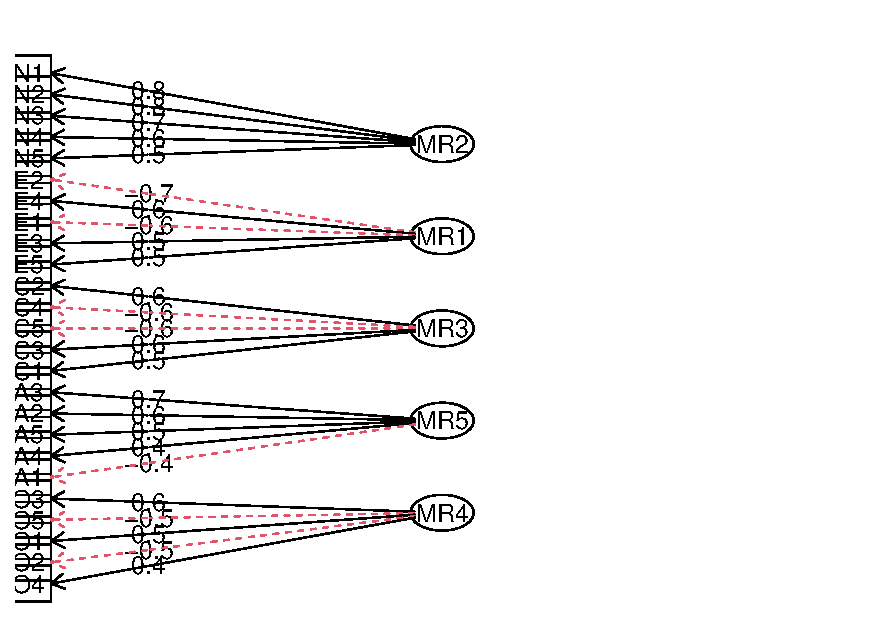
\includegraphics[width=0.3\linewidth]{pics/FA.pdf}	
\end{center}
\end{frame}




\begin{frame}{What factor analysis does well --- and what it misses}
\begin{columns}[T]
\begin{column}{0.48\textwidth}
\begin{block}{Strengths}
\begin{itemize}
    \item compresses many variables into a few hidden factors,
    \item often fits financial or psychometric data well,
    \item gives an interpretable covariance decomposition.
\end{itemize}
\end{block}
\end{column}
\begin{column}{0.48\textwidth}
\begin{block}{Limitations}
\begin{itemize}
    \item loadings are not uniquely identified,
    \item factors are often global rather than local,
    \item the model is covariance-based and may miss multimodality.
\end{itemize}
\end{block}
\end{column}
\end{columns}

\begin{beamercolorbox}[wd=\textwidth,sep=7pt,center,rounded=true,shadow=true]{important}
Factor analysis is good for hidden common shocks, but not for hidden market segments or branching hierarchies.
\end{beamercolorbox}
\end{frame}

% ------------------------------------------------------------
% mixtures
% ------------------------------------------------------------

\section{Latent classes and mixtures}

\begin{frame}[plain,noframenumbering]{}
\begin{center}
{\Huge \textcolor{DarkRed}{Part 2: Gaussian mixtures and latent classes}}
\end{center}
\end{frame}

\begin{frame}{Gaussian mixtures as latent class models}
A Gaussian mixture model has density
\[
p(x)=\sum_{k=1}^K \pi_k \, \phi(x;\mu_k,\Sigma_k),
\qquad
\pi_k\ge 0,
\qquad
\sum_{k=1}^K \pi_k=1.
\]

\begin{block}{Latent class interpretation}
Introduce an unobserved class label $Z\in\{1,\ldots,K\}$ with
\[
\P(Z=k)=\pi_k.
\]
Conditional on $Z=k$, the data come from a Gaussian distribution with parameters $(\mu_k,\Sigma_k)$.
\end{block}

\begin{alertblock}{Economic reading}
A population may consist of hidden segments: conservative vs aggressive investors, low- vs high-productivity firms, or distinct consumer types.
\end{alertblock}
\end{frame}

\begin{frame}{Factor models vs mixture models}
\begin{columns}[T]
\begin{column}{0.48\textwidth}
\begin{block}{Factor model}
A continuous latent variable explains dependence through common shocks.
Observed clouds are typically elongated.
\end{block}
\end{column}
\begin{column}{0.48\textwidth}
\begin{block}{Mixture model}
A discrete latent variable explains dependence through hidden subpopulations.
Observed clouds may be multimodal or clustered.
\end{block}
\end{column}
\end{columns}

\begin{beamercolorbox}[wd=\textwidth,sep=7pt,center,rounded=true,shadow=true]{important}
Continuous latent variables explain \emph{common variation};
 discrete latent variables explain \emph{hidden segmentation}.
\end{beamercolorbox}
\end{frame}

\begin{frame}[fragile]{A Gaussian mixture in \texttt{R}}
\begin{columns}[T,onlytextwidth]
\begin{column}{0.48\textwidth}
\begin{lstlisting}
set.seed(1)
library(mclust)

x1 <- cbind(rnorm(150, -2, 0.8),
            rnorm(150,  0, 0.6))
x2 <- cbind(rnorm(150,  2, 0.8),
            rnorm(150,  1, 0.6))
X <- rbind(x1, x2)
\end{lstlisting}
\end{column}
\begin{column}{0.48\textwidth}
\begin{lstlisting}
fit <- Mclust(X, G = 2)
summary(fit)
plot(fit, what = "classification")
\end{lstlisting}
\end{column}
\end{columns}

\begin{alertblock}{Interpretation}
The hidden label tells us which latent segment generated each observation.
This is a very different explanation of dependence from a factor model.
\end{alertblock}
\end{frame}

\begin{frame}{A quick word on the EM algorithm}
Both factor analysis and Gaussian mixtures are often fitted with versions of the EM algorithm.

\begin{block}{General latent-variable idea}
\begin{itemize}
    \item \textbf{E-step:} estimate the hidden variables given the current parameters,
    \item \textbf{M-step:} update the parameters given the current estimate of the hidden variables.
\end{itemize}
\end{block}

\begin{alertblock}{Examples}
\begin{itemize}
    \item in mixtures, the hidden variable is the class label,
    \item in factor models, the hidden variable is the latent factor vector.
\end{itemize}
\end{alertblock}
\end{frame}

% ------------------------------------------------------------
% latent trees
% ------------------------------------------------------------

\section{Latent trees}

\begin{frame}[plain,noframenumbering]{}
\begin{center}
{\Huge \textcolor{DarkRed}{Part 3: Latent tree models}}
\end{center}
\end{frame}

\begin{frame}{Why latent tree models?}
Sometimes one hidden factor is too crude, but a fully connected latent structure is too complicated.

\begin{columns}[T]
\begin{column}{0.50\textwidth}
\begin{block}{Latent tree idea}
Hidden variables are arranged in a tree, and observed variables appear at the leaves.
\end{block}
\end{column}
\begin{column}{0.45\textwidth}
\begin{block}{Economic reading}
This is natural for hierarchical structures such as sectors, sub-sectors, and firms, or aggregate demand decomposed into regional and local components.
\end{block}
\end{column}
\end{columns}

\begin{beamercolorbox}[wd=\textwidth,sep=7pt,center,rounded=true,shadow=true]{important}
Latent tree models sit between one global factor and a fully general latent network.
\end{beamercolorbox}
\end{frame}

\begin{frame}{A simple latent tree picture}
\begin{center}
\begin{tikzpicture}[>=Latex,scale=0.95,
vertex/.style={circle,draw,very thick,minimum size=6mm,inner sep=0pt},
obs/.style={circle,draw,very thick,minimum size=6mm,inner sep=0pt,fill=blue!12},
lat/.style={circle,draw,very thick,minimum size=6mm,inner sep=0pt,fill=red!18}]

\node[lat] (u0) at (0,2) {$U_0$};
\node[lat] (u1) at (-2,0.8) {$U_1$};
\node[lat] (u2) at (2,0.8) {$U_2$};
\node[obs] (x1) at (-3,-1) {$X_1$};
\node[obs] (x2) at (-1,-1) {$X_2$};
\node[obs] (x3) at (1,-1) {$X_3$};
\node[obs] (x4) at (3,-1) {$X_4$};

\draw[very thick] (u0)--(u1);
\draw[very thick] (u0)--(u2);
\draw[very thick] (u1)--(x1);
\draw[very thick] (u1)--(x2);
\draw[very thick] (u2)--(x3);
\draw[very thick] (u2)--(x4);
\end{tikzpicture}
\end{center}

\begin{alertblock}{Interpretation}
$X_1$ and $X_2$ are similar because they share a local hidden parent $U_1$.
At a higher level, both groups are connected through the root $U_0$.
\end{alertblock}
\end{frame}

\begin{frame}{Why trees are computationally attractive}
Trees are special because many inference problems become simple.

\begin{block}{Message passing intuition}
If the graph has no loops, information can be sent inward from the leaves and outward from the root.
Each local update summarizes everything happening below that node.
\end{block}

\begin{alertblock}{Why this matters}
Belief propagation is exact on trees.
So marginal distributions and conditional probabilities can be computed efficiently even in large latent trees.
\end{alertblock}

\begin{beamercolorbox}[wd=\textwidth,sep=7pt,center,rounded=true,shadow=true]{important}
Trees are beautiful because global inference reduces to local calculations.
\end{beamercolorbox}
\end{frame}

\begin{frame}{Belief propagation in one sentence}
Suppose a tree is rooted at some latent variable.

\begin{columns}[T]
\begin{column}{0.48\textwidth}
\begin{block}{Upward pass}
Each child sends a summary message to its parent.
This message tells the parent how likely different hidden states are, given the evidence below.
\end{block}
\end{column}
\begin{column}{0.48\textwidth}
\begin{block}{Downward pass}
The parent sends back a message combining information from the rest of the tree.
This gives local posterior probabilities at every node.
\end{block}
\end{column}
\end{columns}

\begin{alertblock}{Intuition}
Every message is a compressed summary of a whole subtree.
\end{alertblock}
\end{frame}

\begin{frame}[fragile]{A tiny hidden Markov / tree-flavored example in \texttt{R}}
Even if we do not fit a full latent tree, the computational idea is similar: local hidden states are updated from local evidence.

\begin{columns}[T,onlytextwidth]
\begin{column}{0.48\textwidth}
\begin{lstlisting}
# simple hidden Markov example
library(HMM)
A <- matrix(c(0.9,0.1,
              0.2,0.8), 2, 2,
            byrow = TRUE)
B <- matrix(c(0.8,0.2,
              0.3,0.7), 2, 2,
            byrow = TRUE)
\end{lstlisting}
\end{column}
\begin{column}{0.48\textwidth}
\begin{lstlisting}
hmm <- initHMM(c("low","high"),
               c("bad","good"),
               transProbs = A,
               emissionProbs = B)
forward(hmm, c("good","good",
               "bad","good"))
\end{lstlisting}
\end{column}
\end{columns}

\begin{alertblock}{Interpretation}
The same message-passing idea underlies more general tree-structured latent models.
\end{alertblock}
\end{frame}

% ------------------------------------------------------------
% RBM
% ------------------------------------------------------------

\section{Restricted Boltzmann machines}

\begin{frame}[plain,noframenumbering]{}
\begin{center}
{\Huge \textcolor{DarkRed}{Part 4: Restricted Boltzmann machines}}
\end{center}
\end{frame}

\begin{frame}{Restricted Boltzmann machines}
A restricted Boltzmann machine (RBM) is a bipartite latent-variable model with visible units $x$ and hidden units $h$.

\begin{center}
\begin{tikzpicture}[>=Latex,scale=0.95,
vis/.style={circle,draw,very thick,minimum size=6mm,fill=blue!12},
lat/.style={circle,draw,very thick,minimum size=6mm,fill=red!18}]
\node[vis] (x1) at (0,0) {$x_1$};
\node[vis] (x2) at (1.2,0) {$x_2$};
\node[vis] (x3) at (2.4,0) {$x_3$};
\node[vis] (x4) at (3.6,0) {$x_4$};
\node[lat] (h1) at (0.8,1.6) {$h_1$};
\node[lat] (h2) at (2.8,1.6) {$h_2$};
\foreach \u in {x1,x2,x3,x4}
  {\draw[very thick] (\u)--(h1);
   \draw[very thick] (\u)--(h2);} 
\end{tikzpicture}
\end{center}

\begin{alertblock}{Restriction}
There are no visible-visible edges and no hidden-hidden edges.
This makes conditional distributions very simple.
\end{alertblock}
\end{frame}

\begin{frame}{Why RBMs matter here}
RBMs are still latent-variable models, but they point toward neural networks.

\begin{block}{Modeling idea}
The hidden units capture a distributed latent representation of the visible variables.
Unlike a classical one-factor model, many hidden units can be active at once.
\end{block}

\begin{columns}[T]
\begin{column}{0.48\textwidth}
\begin{block}{Classical latent models}
\begin{itemize}
    \item one or a few interpretable latent variables,
    \item emphasis on structure and interpretation.
\end{itemize}
\end{block}
\end{column}
\begin{column}{0.48\textwidth}
\begin{block}{RBMs / deep learning bridge}
\begin{itemize}
    \item many hidden features,
    \item emphasis on representation rather than interpretation.
\end{itemize}
\end{block}
\end{column}
\end{columns}
\end{frame}

\begin{frame}{From RBMs to sigmoid activation}
For a binary RBM, the joint distribution has the form
\[
P(x,h) \propto \exp\!\left( a^\top x + b^\top h + x^\top W h \right).
\]
Because the graph is bipartite,
\[
P(h_j=1\mid x)
= \frac{\exp(b_j + w_j^\top x)}{1+\exp(b_j + w_j^\top x)}
= \sigma(b_j+w_j^\top x),
\]
where $\sigma(t)=1/(1+e^{-t})$ is the sigmoid function.

\begin{alertblock}{Bridge to neural nets}
A hidden unit in an RBM activates according to a sigmoid of a linear score.
This is one reason RBMs historically formed a bridge from latent-variable models to neural-network representations.
\end{alertblock}
\end{frame}

\begin{frame}[fragile]{A tiny RBM-style code illustration}
In modern practice, one usually works with autoencoders or neural nets rather than classical RBM training, but the basic hidden-layer idea is similar.

\begin{columns}[T,onlytextwidth]
\begin{column}{0.48\textwidth}
\begin{lstlisting}
set.seed(1)
X <- matrix(rbinom(500*4, 1, 0.5),
            500, 4)
W <- matrix(c(1.2,-0.8,
              0.5, 1.1,
             -0.7, 0.9,
              1.0, 0.6), 4, 2,
            byrow = TRUE)
\end{lstlisting}
\end{column}
\begin{column}{0.48\textwidth}
\begin{lstlisting}
eta <- X %*% W
Hprob <- 1/(1 + exp(-eta))
head(Hprob)
\end{lstlisting}
\end{column}
\end{columns}

\begin{alertblock}{Interpretation}
The hidden layer turns observed inputs into latent activation probabilities --- the modern representation-learning version of a latent-variable model.
\end{alertblock}
\end{frame}

% ------------------------------------------------------------
% closing
% ------------------------------------------------------------

\section{Conclusion}

\begin{frame}{Take-away}
\begin{itemize}
    \item Factor analysis explains dependence through a few hidden common shocks.
    \item Gaussian mixtures explain dependence through hidden subpopulations.
    \item Latent tree models explain dependence through hierarchical hidden structure.
    \item Message passing makes tree-structured inference computationally attractive.
    \item RBMs show how latent-variable ideas connect naturally to neural-network representations.
\end{itemize}

\vspace{2mm}
\begin{beamercolorbox}[wd=\textwidth,sep=8pt,center,rounded=true,shadow=true]{important}
Different latent models explain dependence in different ways:
common factors, hidden classes, hierarchies, or distributed features.
\end{beamercolorbox}
\end{frame}

\begin{frame}{Looking ahead}
\begin{block}{Next lecture}
We will return to hidden variables from a more causal perspective: unobserved confounding, proxy controls, and what survives when the clean DAG picture breaks.
\end{block}

\begin{alertblock}{Bridge forward}
Today the latent variables explained dependence.
Next time they will also threaten identification.
\end{alertblock}
\end{frame}

\end{document}
